\section{Process Models}
%Providing process models is not enough because the process owner is diffident with any result which he/she is simply provided with. Therefore, he/she wants evidence of the goodness of these models. For this purpose, you should perform alignment-based conformance checking. Using the result of the conformance checker, you should motivate why the chosen models are better that any possible alternative (e.g. because of mediating fitness, precision, generalization and simplicity). For each model, also provide its textual description. 

\subsection{Exploring process}

For exploring a good model of a data set I first filtered the data with the (\textbf{Filter log on event attribute names}) tool for extracting the required. Then I used \textbf{Interactive data heuristic miner} and \textbf{Inductive Miner} on the filtered data set to discover different models. After comparing the outcomes I decided to concentrate on \textbf{Interactive data heuristic miner} and their directly followed graphs and petri nets for understanding the lifecycle. I think the directly followed graph is the best, but for checking the model I also checked the petri net with corresponding frequency filtering and basis configuration. The conformance checking where done with \textbf{Replay a log on Petri Net for conformance analysis} tool on the petri net and the filtered data. For the precision check I applied the \textbf{Multi-perspective Process Explorer} tool on the petri net and the filtered data and chose "show precision mode" in the tool with basic configuration.

\subsection{Application data set}
%filter on event names
%interactive data heuristic miner oder inductive minder und dann petri net
%conformance 
%multi-perspective
Just the events beginning with "App\_..." are required. The resulting data set is saved as "Filtered App".

\subsubsection{General details of the data set}

The data set is collected between 1st of 0ct 2011 (saturday), 00:38:44 and 14th of Mar 2012 (Wednesday), 15:33:57. It contains 13087 cases with 60849 executed events.

10 different events appear: "App\_Fully\_Submission" (21.507\%), "App\_Incomplete\_Submission" (21.507\%), "App\_Rejection" (12.547\%), "App\_Pre\_Acceptation" (12.107\%), "App\_Acceptation" (8.403\%), ("App\_Finalization" (8.242\%), "App\_Cancellation" (4.613\%), "App\_Initiation" (3.691\%), "App\_Approving" (3.691\%) and "App\_Registration" (3.691\%). Just "APP\_Fully\_Submission" appears to be a start event. However there are 8 end events possible: "App\_Rejection" (58.34\%), "App\_Cancellation" (21.449\%), "App\_Initiation" (8.573\%), "App\_Registration" (6.014\%), "App\_Approving" (2.575\%), "App\_Finalization" (2.499\%), "App\_Pre\_Acceptation" (0.527\%) and "App\_Acceptation" (0.023\%).

A trace contains maximal 8 different events and minimal 3. The mean is 4.65. In total there are 17 different variants of traces. 


\begin{figure}[!htbp]
\centering
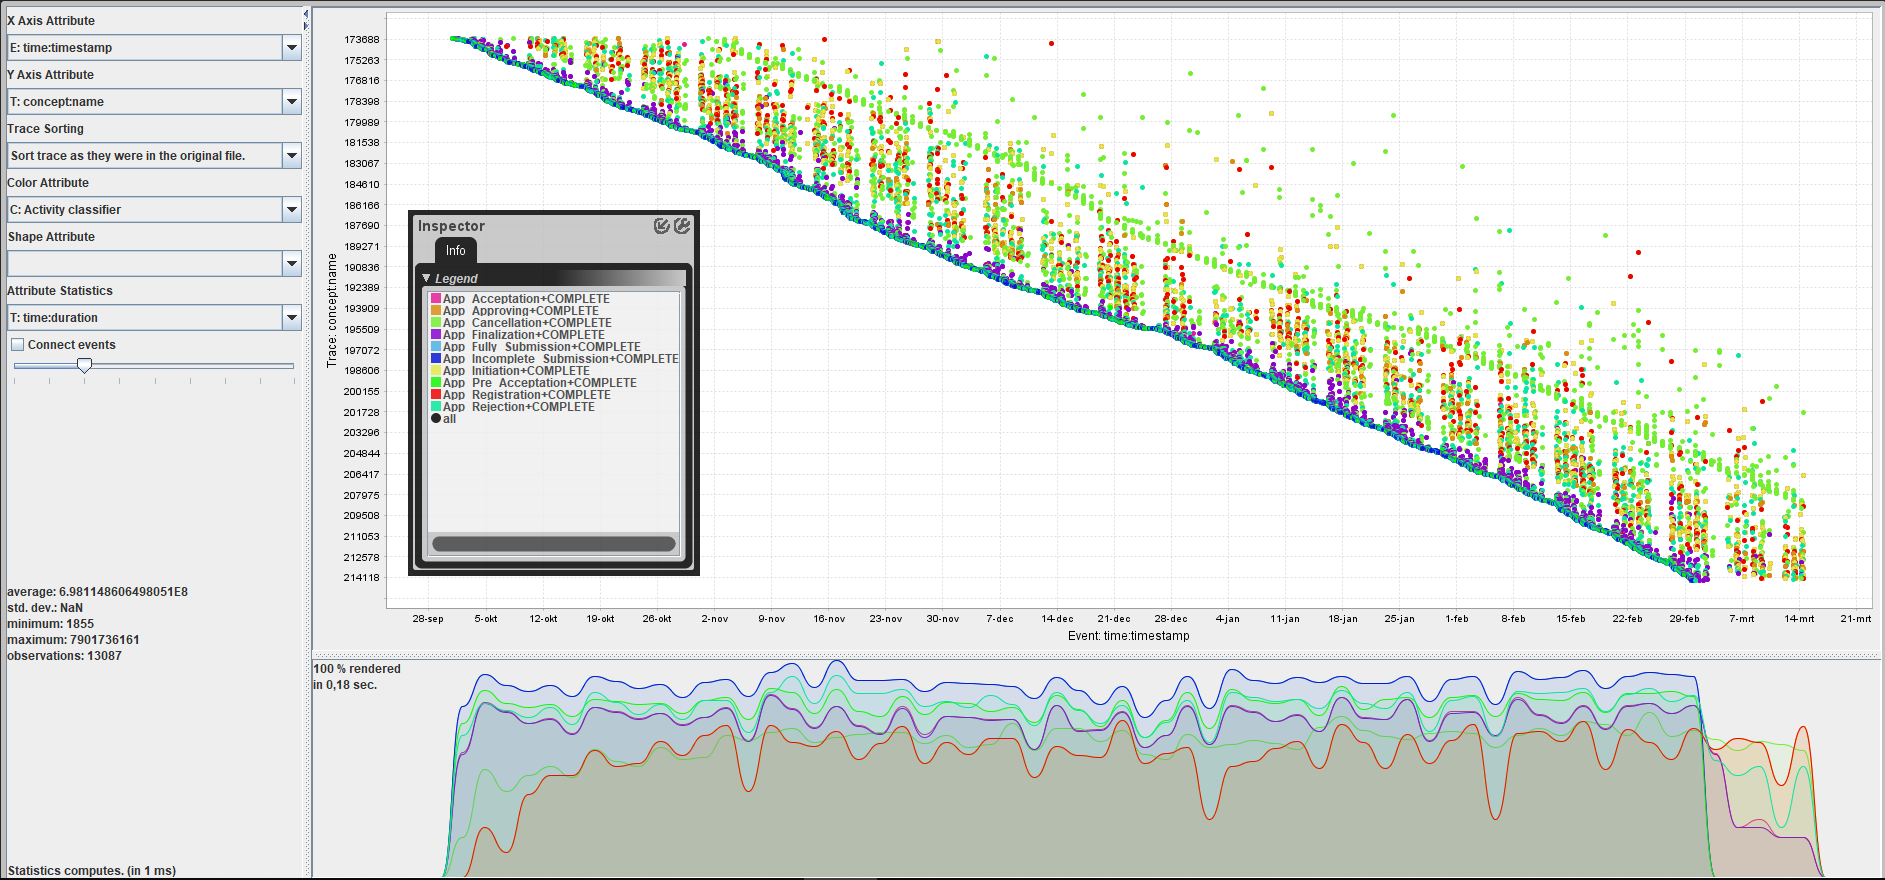
\includegraphics[height = 0.2\textheight]{AppData.PNG}
\caption{Dotted chart showing the time of events}
\label{fig:AppTimeFlow}
\end{figure}

In figure \ref{fig:AppTimeFlow} the dotted chart can be seen. Having a closer look at this chart you see gaps, which are always on a sunday. Those gaps do not appear for "APP\_Pre\_Acceptation" and "APP\_Incomplete\_Submission". Furthermore is in the left below corner to see the average duration of a case, 8 days 1 hours 55 minutes and 14.86 seconds, and the maximum duration, 91 days 10 hours 55 minutes and 36.16 seconds. Both are given in milliseconds.


\subsubsection{Discover and evaluate a model of the application lifecycle}

\begin{figure}[!htbp]
\centering
\begin{subfigure}{.4\textwidth}
  \centering
  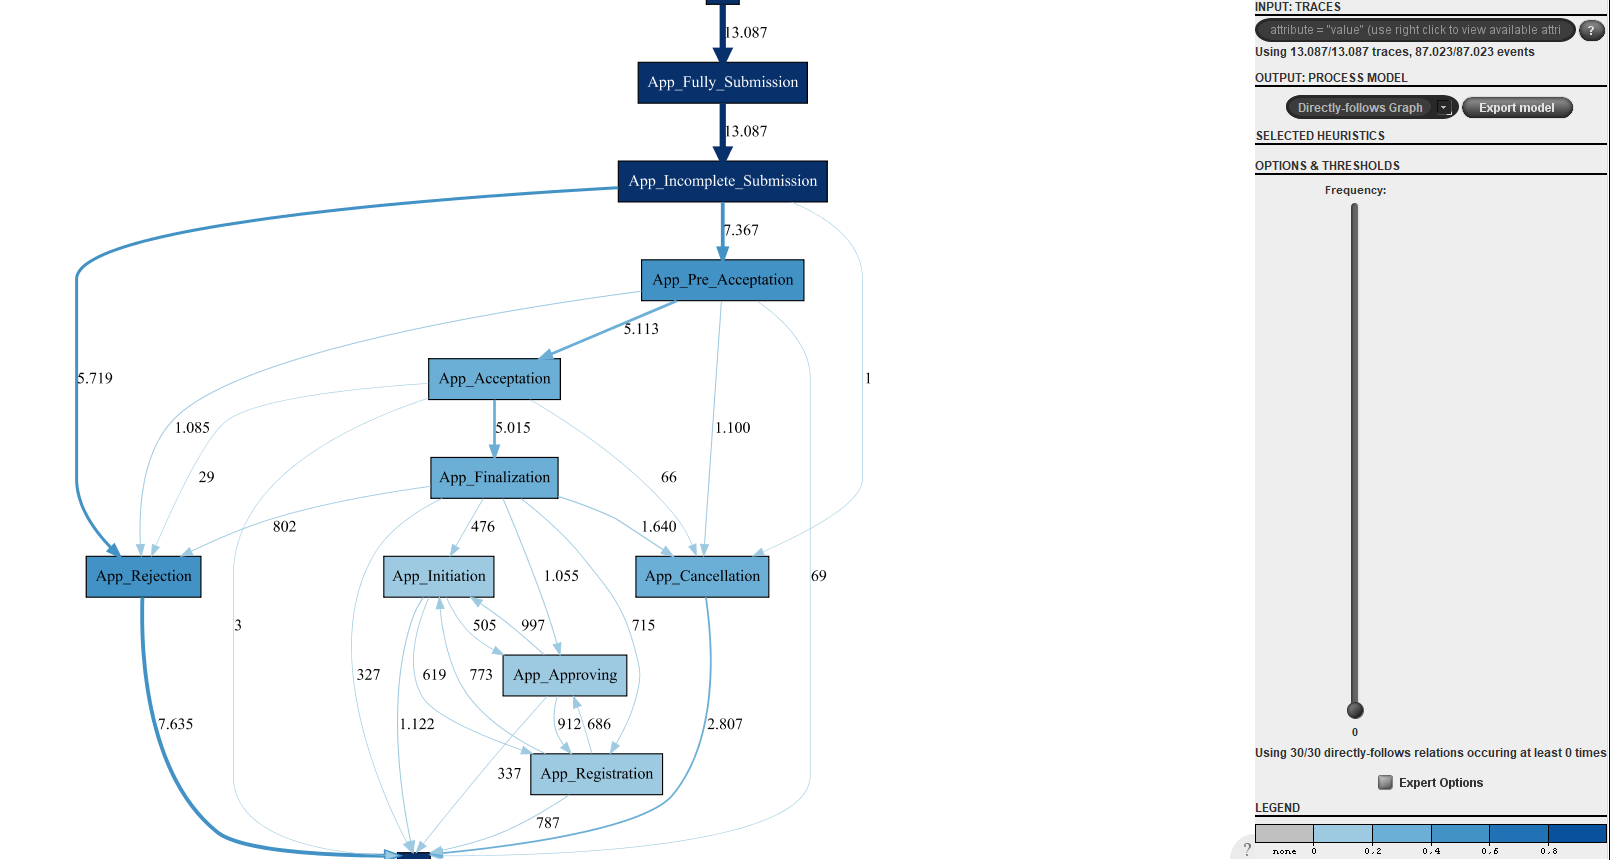
\includegraphics[width=\linewidth]{App_DirectlyFollowedFreq0.PNG}
  \caption{Directly followed graph without frequency filtering}
  \label{fig:APP_DFG0}
\end{subfigure}%
\begin{subfigure}{.4\textwidth}
  \centering
  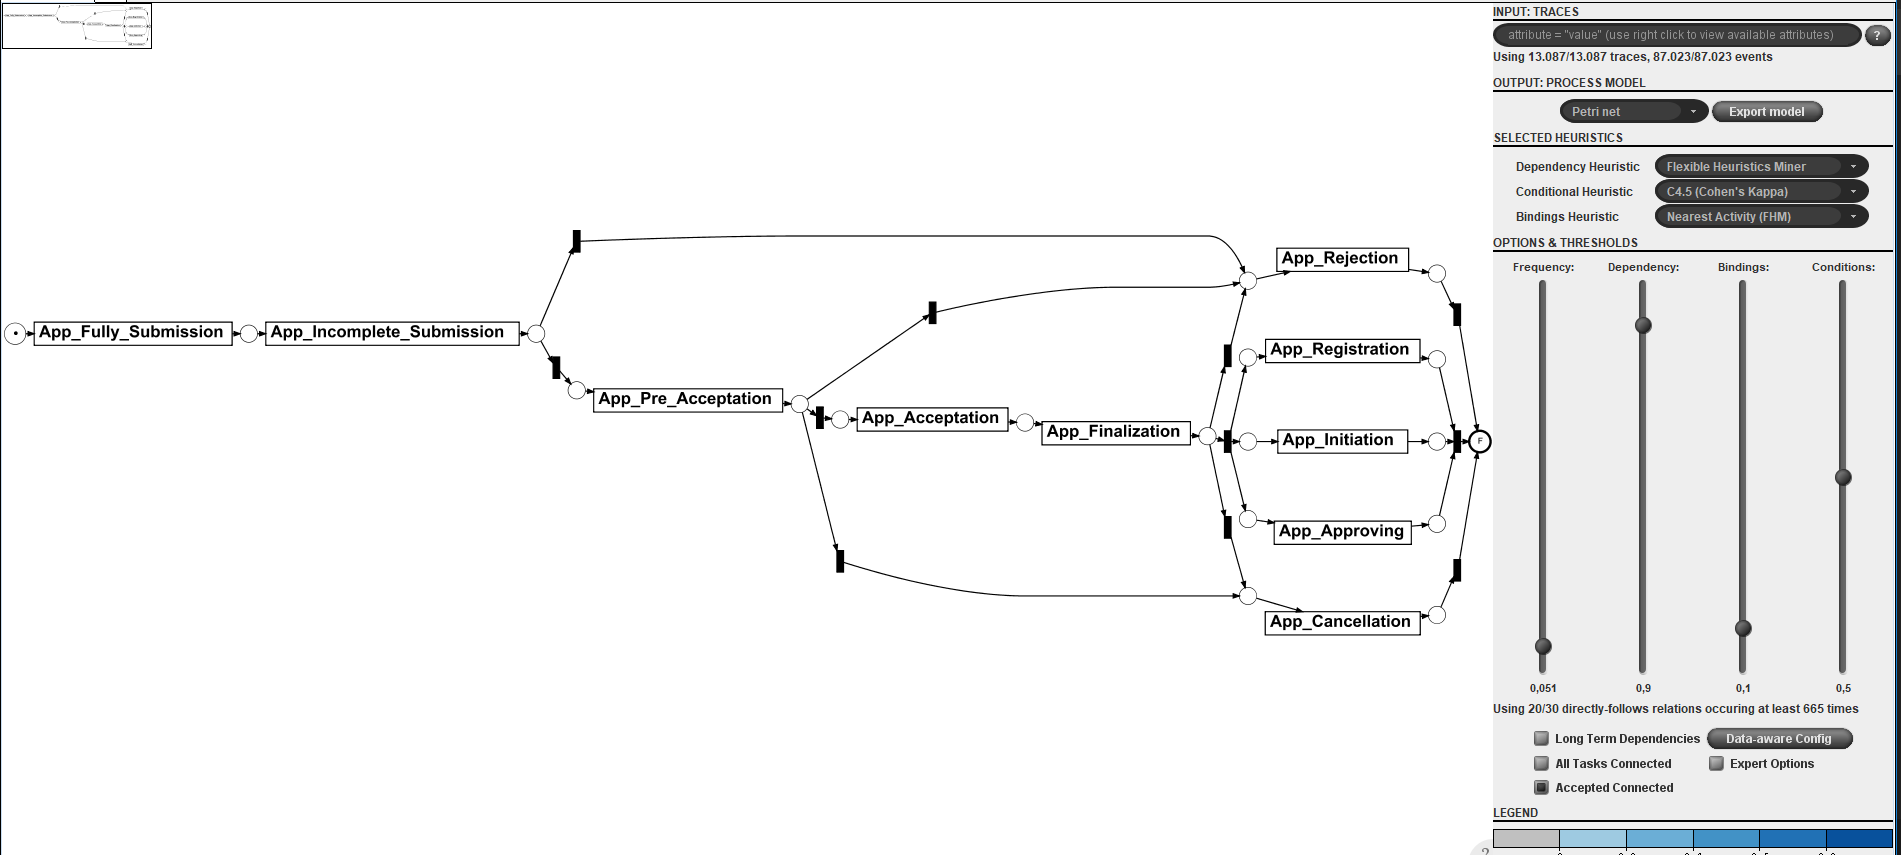
\includegraphics[width=\linewidth]{App_DirectlyFollowedFreq0-051.PNG}
  \caption{Directly followed graph 0.051 frequency}
  \label{fig:APP_DFG0-51}
\end{subfigure}
\begin{subfigure}{.4\textwidth}
  \centering
  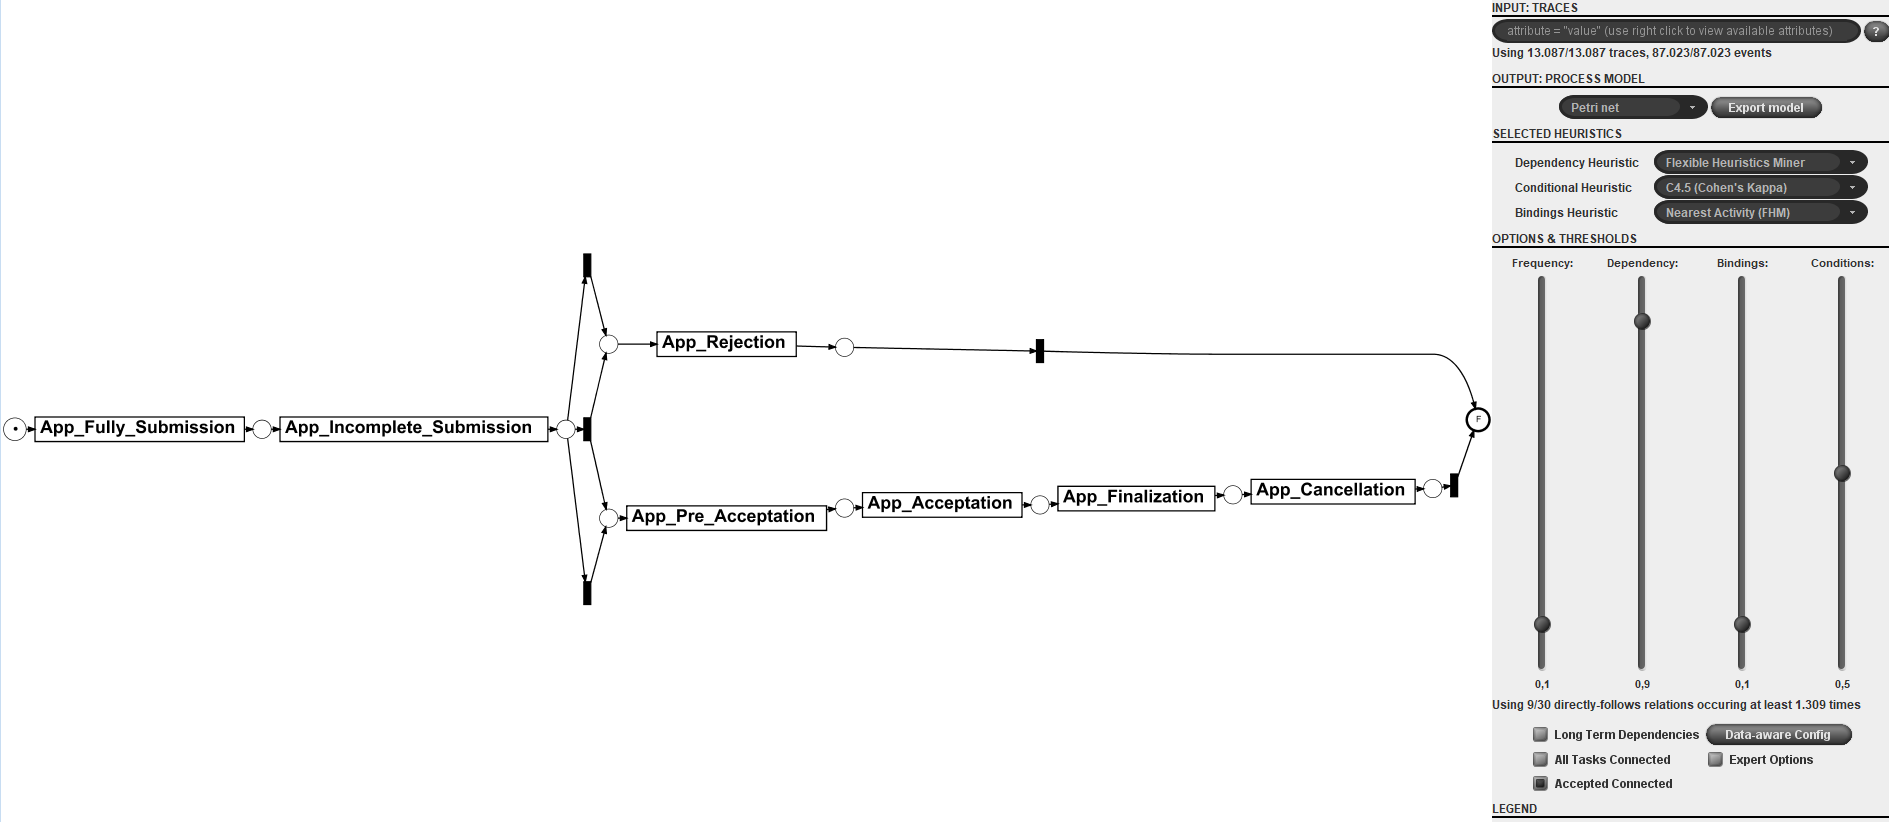
\includegraphics[width=\linewidth]{App_DirectlyFollowedFreq0-1.PNG}
  \caption{Directly followed graph 0.1 frequency}
  \label{fig:APP_DFG0-1}
\end{subfigure}
\begin{subfigure}{.4\textwidth}
  \centering
  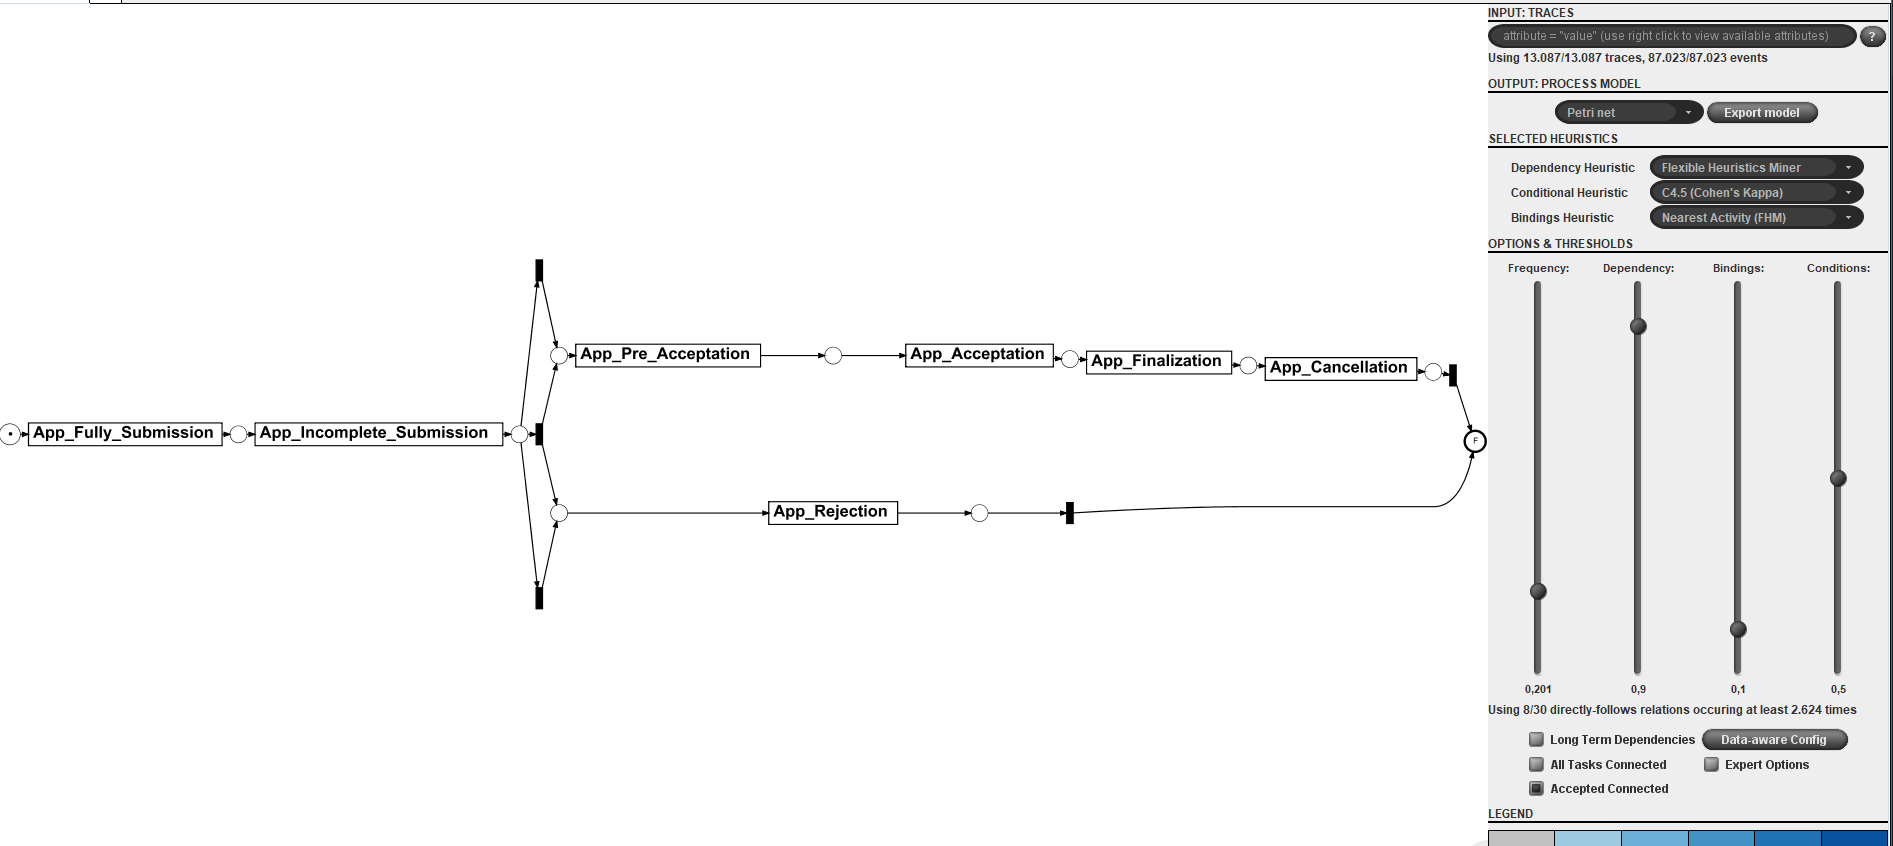
\includegraphics[width=\linewidth]{App_DirectlyFollowedFreq0-2.PNG}
  \caption{Directly followed graph 0.2 frequency}
  \label{fig:APP_DFG0-2}
\end{subfigure}
\caption{Considered directly followed graphs}
\label{fig:App_Direct}
\end{figure}

To find an accurate model I tried different frequency filters. First I chose the frequency 0.1 and had a look at the directly followed graph. I also checked 0.2 and 0.51. For comparsion in the end I had also a look at the original directly followed graph found by the \textbf{Interactive data heuristic miner}. In figure \ref{fig:App_Direct} the 4 considered directly followed graphs can be seen. My first choice was the directly followed graph with 0.1 as threhold for frequency, because it was a simple model that still tells us a lot about the main process and is not to specific (still has an acceptable generalization). Obviously the original graph does not fullfill the criterium of simplicity and also the graph with frequency 0.051 still looks not simple enough.

\begin{figure}[!htbp]
\centering
\begin{subfigure}{.25\textwidth}
  \centering
  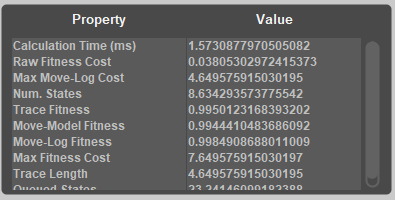
\includegraphics[width=\linewidth]{App_Conformance0-051.PNG}
  \caption{Conformance for 0.051 frequency}
  \label{fig:APP_Conf0-051}
\end{subfigure}%
\begin{subfigure}{.25\textwidth}
  \centering
  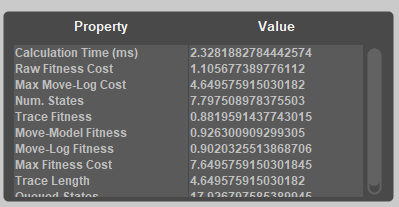
\includegraphics[width=\linewidth]{App_Conformance0-1.PNG}
  \caption{Conformance 0.1}
  \label{fig:APP_Conf0-1}
\end{subfigure}
\begin{subfigure}{.25\textwidth}
  \centering
  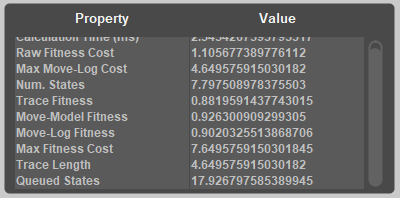
\includegraphics[width=\linewidth]{App_Conformance0-2.PNG}
  \caption{Conformance for 0.2 frequency}
  \label{fig:APP_Conf0-2}
\end{subfigure}
\caption{Conformance checking}
\label{fig:App_Conf}
\end{figure}

In the next step I checked the conformance of the corresponding petri nets (using basic configuration just changing the frequency filter), which I exported from the Interactive \textbf{Data-aware Heuristic Miner}, by combining the data and the petri net for the conformance checking with the \textbf{Replay a log on Petri Net for conformance analysis} tool. 

The results are shown in figure \ref{fig:App_Conf}. To see is that the model with 0.2 also has the same conformanc outcome as 0.1, what is not surprising since I have the same petri-net for the configuration I used. Based on the simplicity and generalization and the fact, that the fitness of 0.1 filtering is still not bad (88.20\% fitness) I considered 0.051 and 0.1 for the precision check.

For the precision check I applied the \textbf{Multi-perspective Process Explorer} tool and chose "show precision mode" in the tool with simple configuration.

\begin{figure}[!htbp]
\centering
\begin{subfigure}{.4\textwidth}
  \centering
  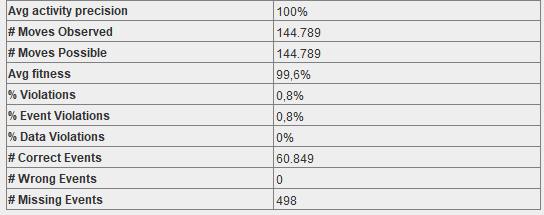
\includegraphics[width=\linewidth]{App_Precision0-051.PNG}
  \caption{Precision for 0.051 as frequency}
  \label{fig:APP_Prec0-051}
\end{subfigure}%
\begin{subfigure}{.4\textwidth}
  \centering
  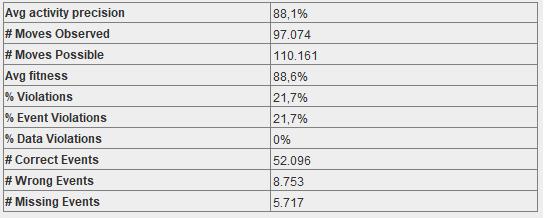
\includegraphics[width=\linewidth]{App_Precision0-1.PNG}
  \caption{Precision for 0.1 as frequency}
  \label{fig:APP_Prec0-1}
\end{subfigure}
\caption{Precision checking}
\label{fig:App_Prec}
\end{figure}

%0.07
Having a look at the precision, figure \ref{fig:App_Prec}, I could see, that the precision of 0.51 filtering is 100\%, but of the 0.1 filtering just 88.1\%. In combination with the results before, I came to the conclusion, that 0.1 filtering is not good enough as model and 0.051 would be good enough, but did not fullfill my simplicity criterium. Starting by this I again tried different frequency filters starting by 0.075 to find a model fullfilling both, a similar simplicity as the 0.1 frequency model, but a better conformance and precision than this simpel model. Already the frequency filtering 0.076 gives me the wished result.

\begin{figure}[!htbp]
\centering
\begin{subfigure}{.4\textwidth}
  \centering
  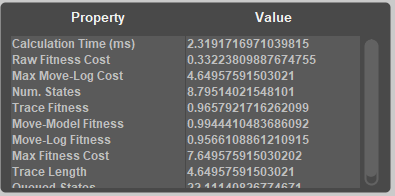
\includegraphics[width=\linewidth]{App_Conformance0-076.PNG}
  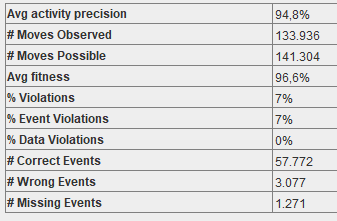
\includegraphics[width=\linewidth]{App_Precision0-076.PNG}
  \caption{Conformance and Precision}
  \label{fig:APP_Conf0-076}
\end{subfigure}
\begin{subfigure}{0.5\textwidth}
  \centering
  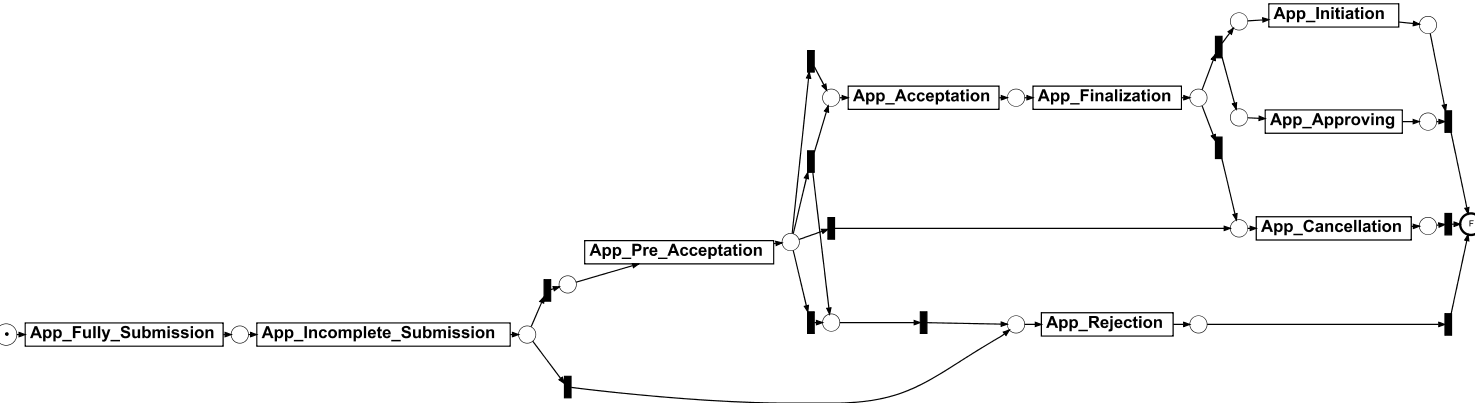
\includegraphics[height=0.3\textheight]{App_DirectlyFollowedFreq0-076.PNG}
  \caption{Directly followed graph}
  \label{fig:APP_DF0-076}
\end{subfigure}%
\caption{Frequency 0.076}
\label{fig:App_Prec}
\end{figure}

This model has a good simplicity, but still has a path fitness of 96.58\% and precision of 94.8\%, so it is still pretty good. Overall I so decided to choose the 0.076 frequency model for the application's lifecycle.

The process always starts with "App\_Fully\_Submission" and "App\_Incomplete\_Submission". After all 13087 cases completeted this two steps, 7367, roughly spoken 50\%, accomplished "App\_Pre\_Acceptation". They now split again, where the most cases continue with App\_Acceptation (5113 cases) and then App\_Finalization (5015 cases). App\_Pre\_Acceptation is second most followed by App\_Cancellation (1100 cases, which is a fifth of the amount of cases for App\_Acceptation) and the last possibility is App\_Rejection (1085 cases). App\_Finalization also has two different followed actions, App\_Approving (1055 cases) and App\_Cancellation (1640 cases coming from App\_Finalization). App\_Cancellation thus is been performed in 2740 cases by the pathes to see, but in total by 2807. App\_Approving is been followed by App\_Initiation in 997 cases, but App\_Initiation is executed 1122 times. App\_Rejection has the predecessor actions as explained above in 6804 cases, but in total is been done in 7635 cases. 

All the differences between incoming and outcoming cases can be explained by the filtering of the frequency. Because of this filtering not all possible pathes are visible, but just the 92.4\% most common ones.

\subsection{Proposal data}

\subsubsection{General Details of the data set}
The data set is collected between 1st of 0ct 2011 (saturday), 10:44:40 and 14th of Mar 2012 (Wednesday), 15:50:59. Having a look at the visualization you can see that there a gaps in the workflow. 

\begin{figure}[!htbp]
\centering
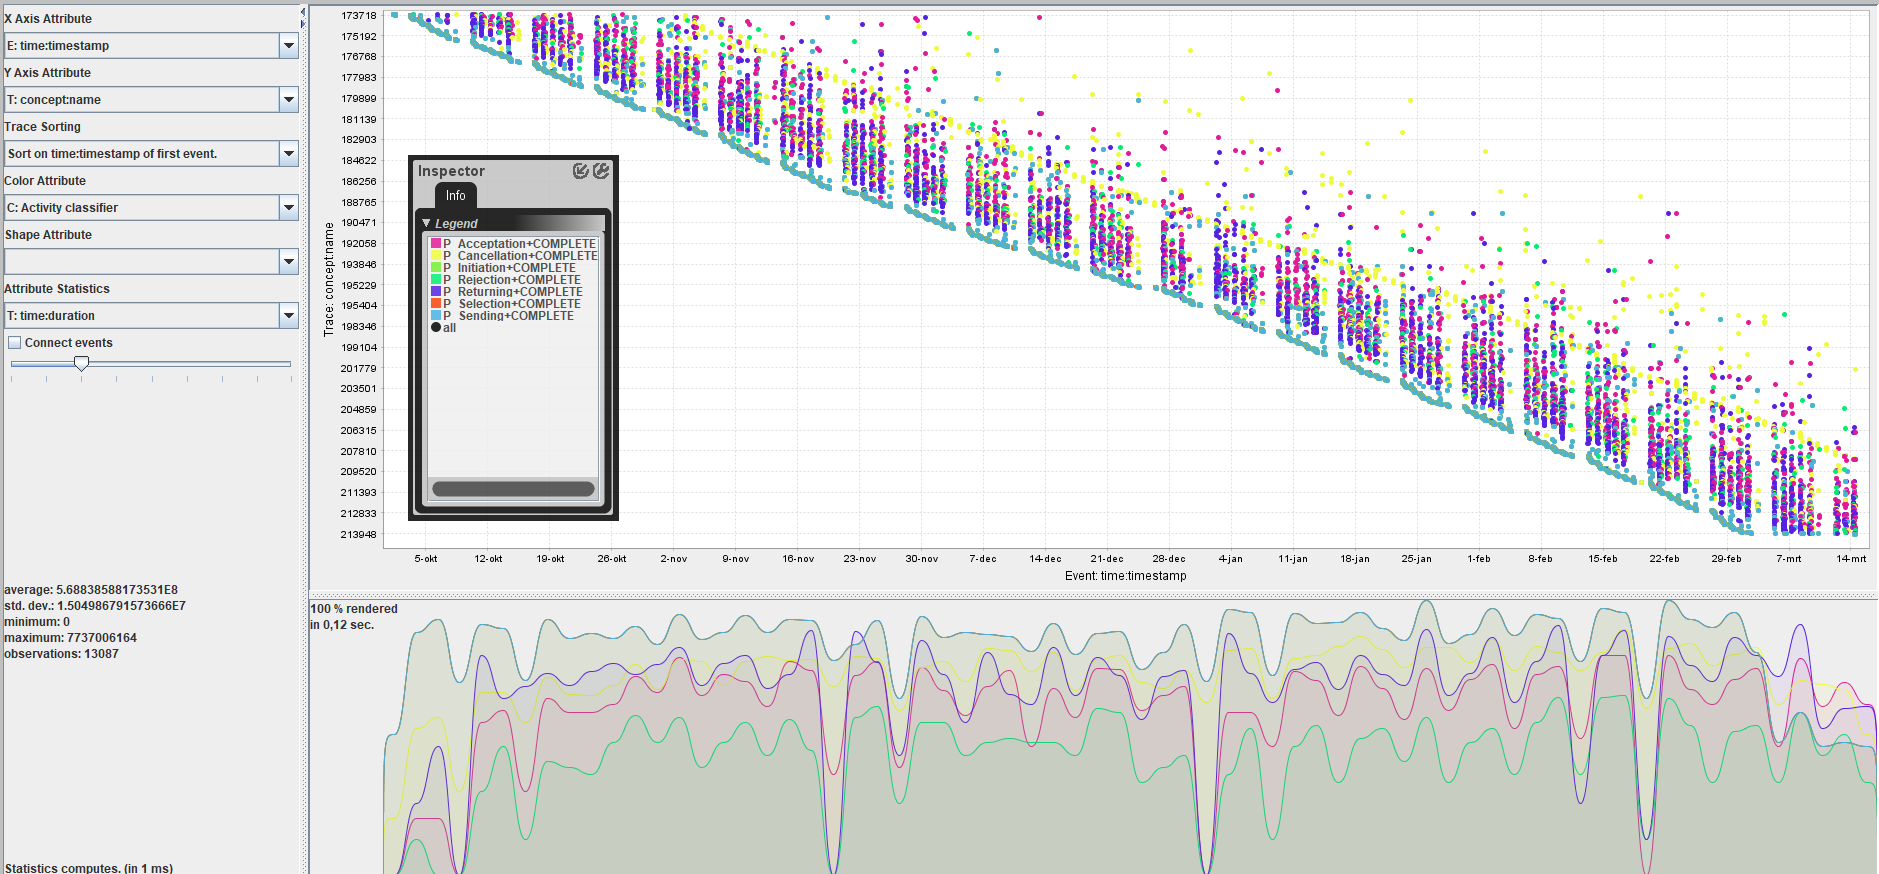
\includegraphics[height = 0.2\textheight]{ProposalData.PNG}
\caption{Dotted chart showing the time of events}
\label{fig:PropTimeFlow}
\end{figure}

In figure \ref{fig:PropTimeFlow} the dotted chart can be seen. Having a closer look at this gaps makes clear, that it is always a sunday. What does not show this behavior so clear is "P\_Cancellation" and "P\_Initiation". Furthermore is in the left below corner to see what is the average duration of a case, 65 days 20 hours 6 minutes and 25.88 seconds, and the maximum duration, 89 days 13 hours 10 minutes and 6.16 seconds. Both is given in milliseconds.

The data set has 7 events: "P\_Initiation" (22.5\%), 
"P\_Sending" (22.5\%), "P\_Selection" (22.5\%), "P\_Cancellation" (11.698\%), "P\_Returning" (11.055\%), "P\_Acceptation"(7.179\%) and "P\_Rejection" (2.567\%), where the percentage is the relative occurence. In total this data set contains 13087 cases with in total 31244 events. It always stars with "P\_Selection" and has 5 different end events: "P\_Acceptation" (44.726\%), "P\_Cancellation"(32,702\%), "P\_Rejection" (15.992\%), "P\_Sending" (4.806\%) and "P\_Returning" (1.775\%).

There are 169 different variants of traces.

Maximal 30 events are executed in a class of cases and minimal 0, what is a hint, that there are cases ending directly. The mean of events per class is 2.387.


\subsubsection{Discover and evaluate a model of the proposal lifecycle}

Applying the steps on the proposal data set it gave me 4 models I wanted to have a closer look at.

\begin{figure}[!htbp]
\centering
\begin{subfigure}{.4\textwidth}
  \centering
  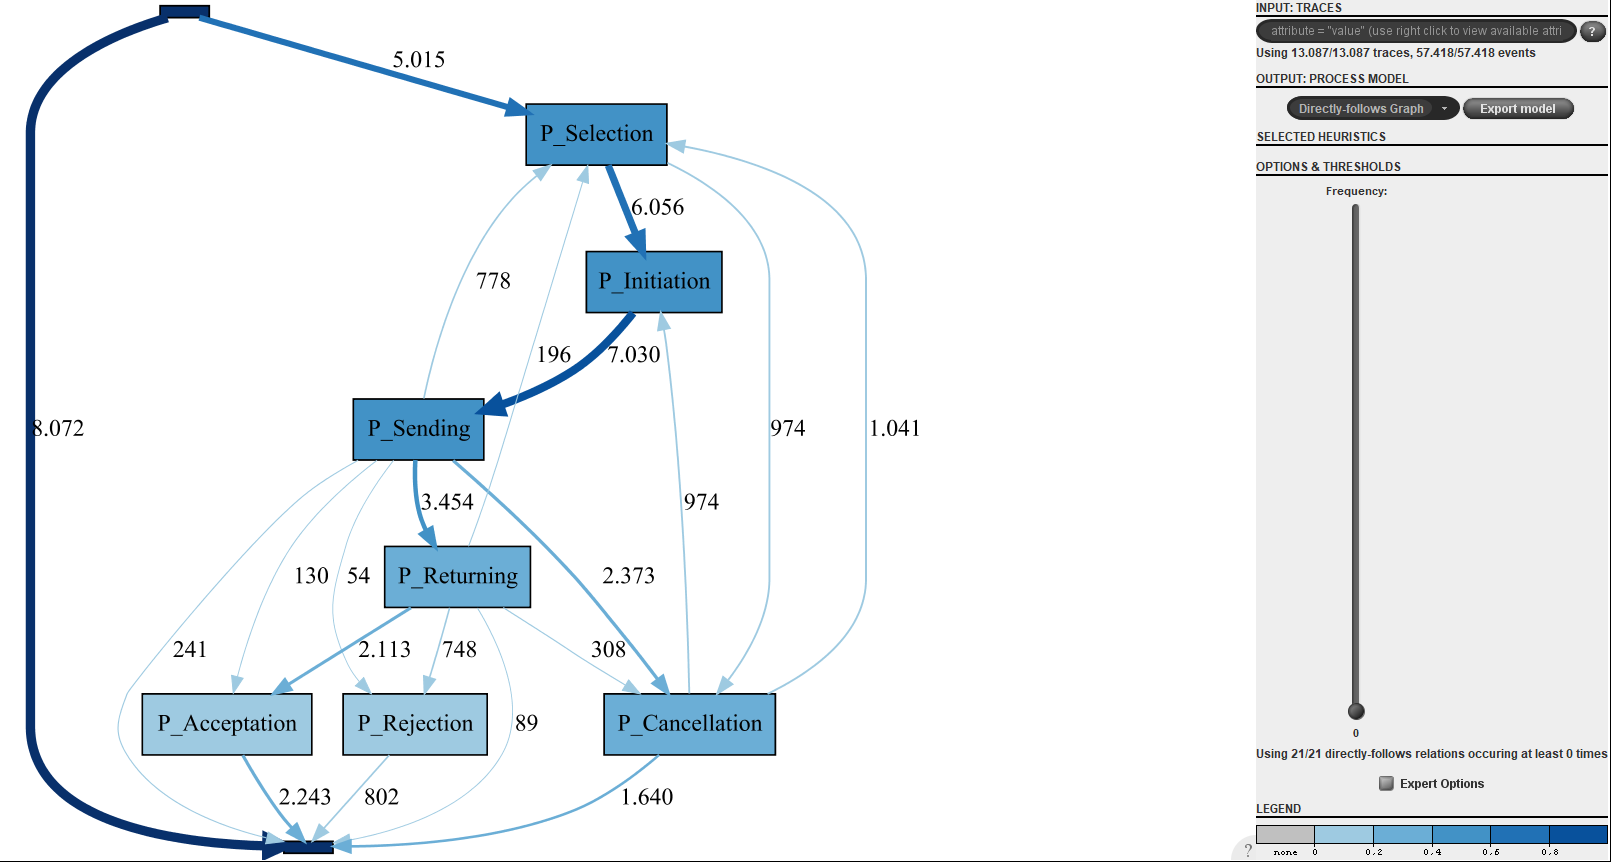
\includegraphics[width=\linewidth]{P_DirectlyFollowedFreq0.PNG}
  \caption{Directly followed graph without frequency filtering}
  \label{fig:P_DFG0}
\end{subfigure}%
\begin{subfigure}{.4\textwidth}
  \centering
  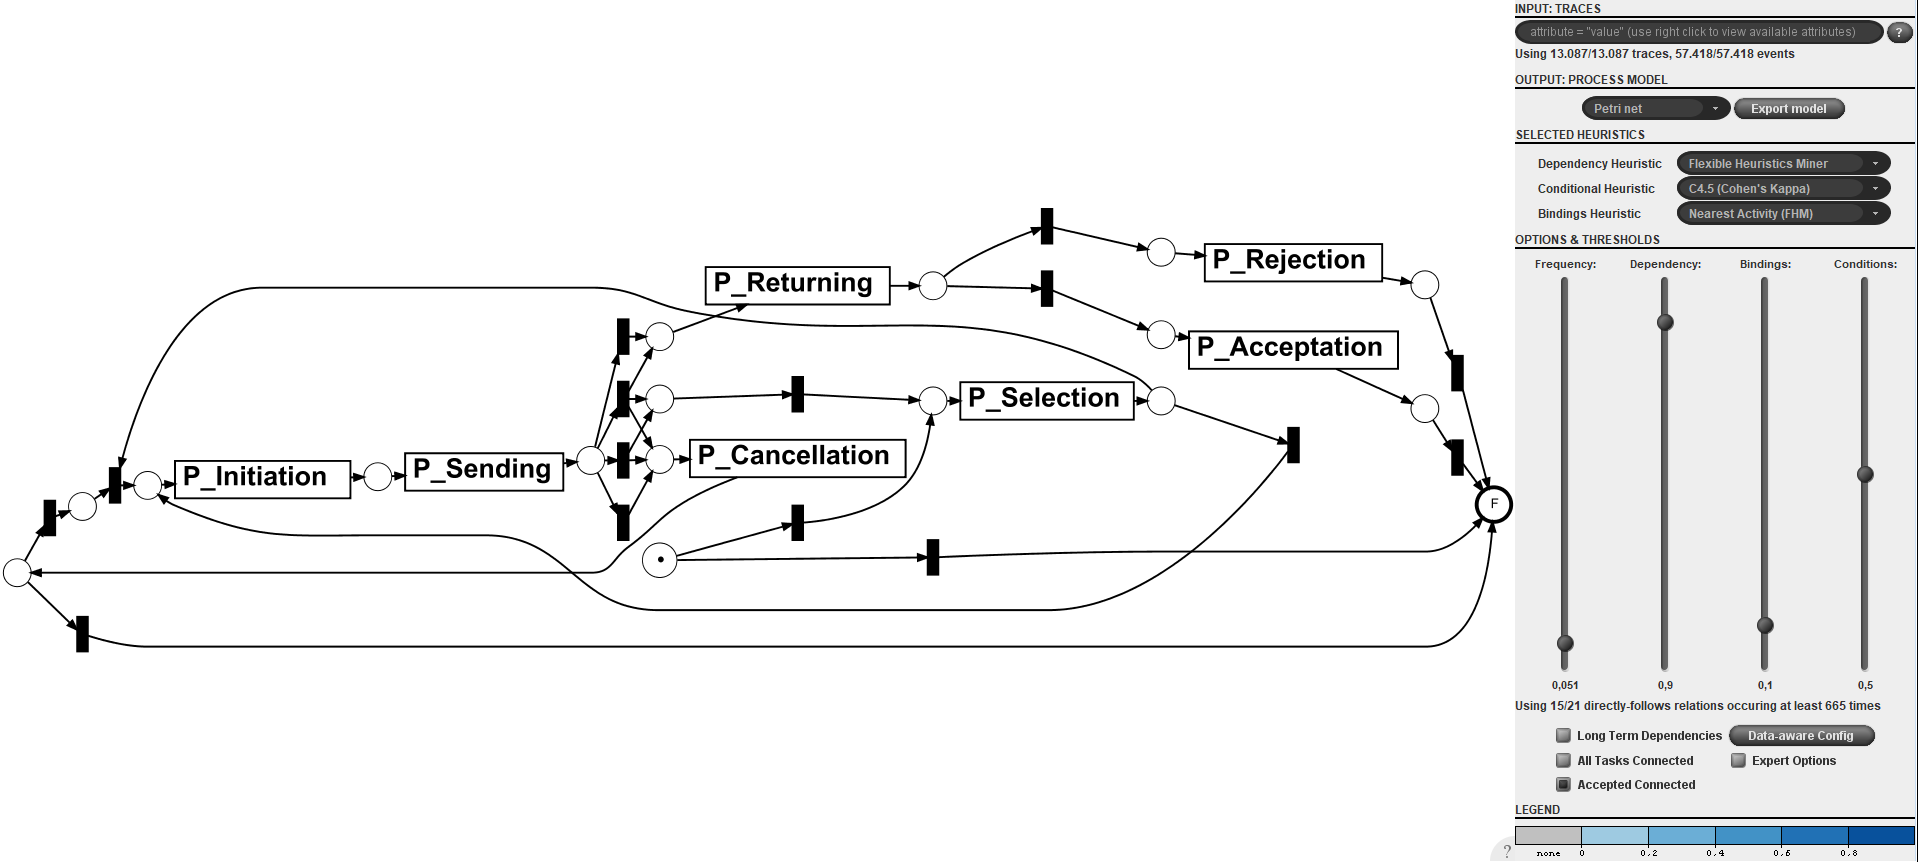
\includegraphics[width=\linewidth]{P_DirectlyFollowedFreq0-051.PNG}
  \caption{Directly followed graph 0.051 frequency}
  \label{fig:P_DFG0-051}
\end{subfigure}
\begin{subfigure}{.4\textwidth}
  \centering
  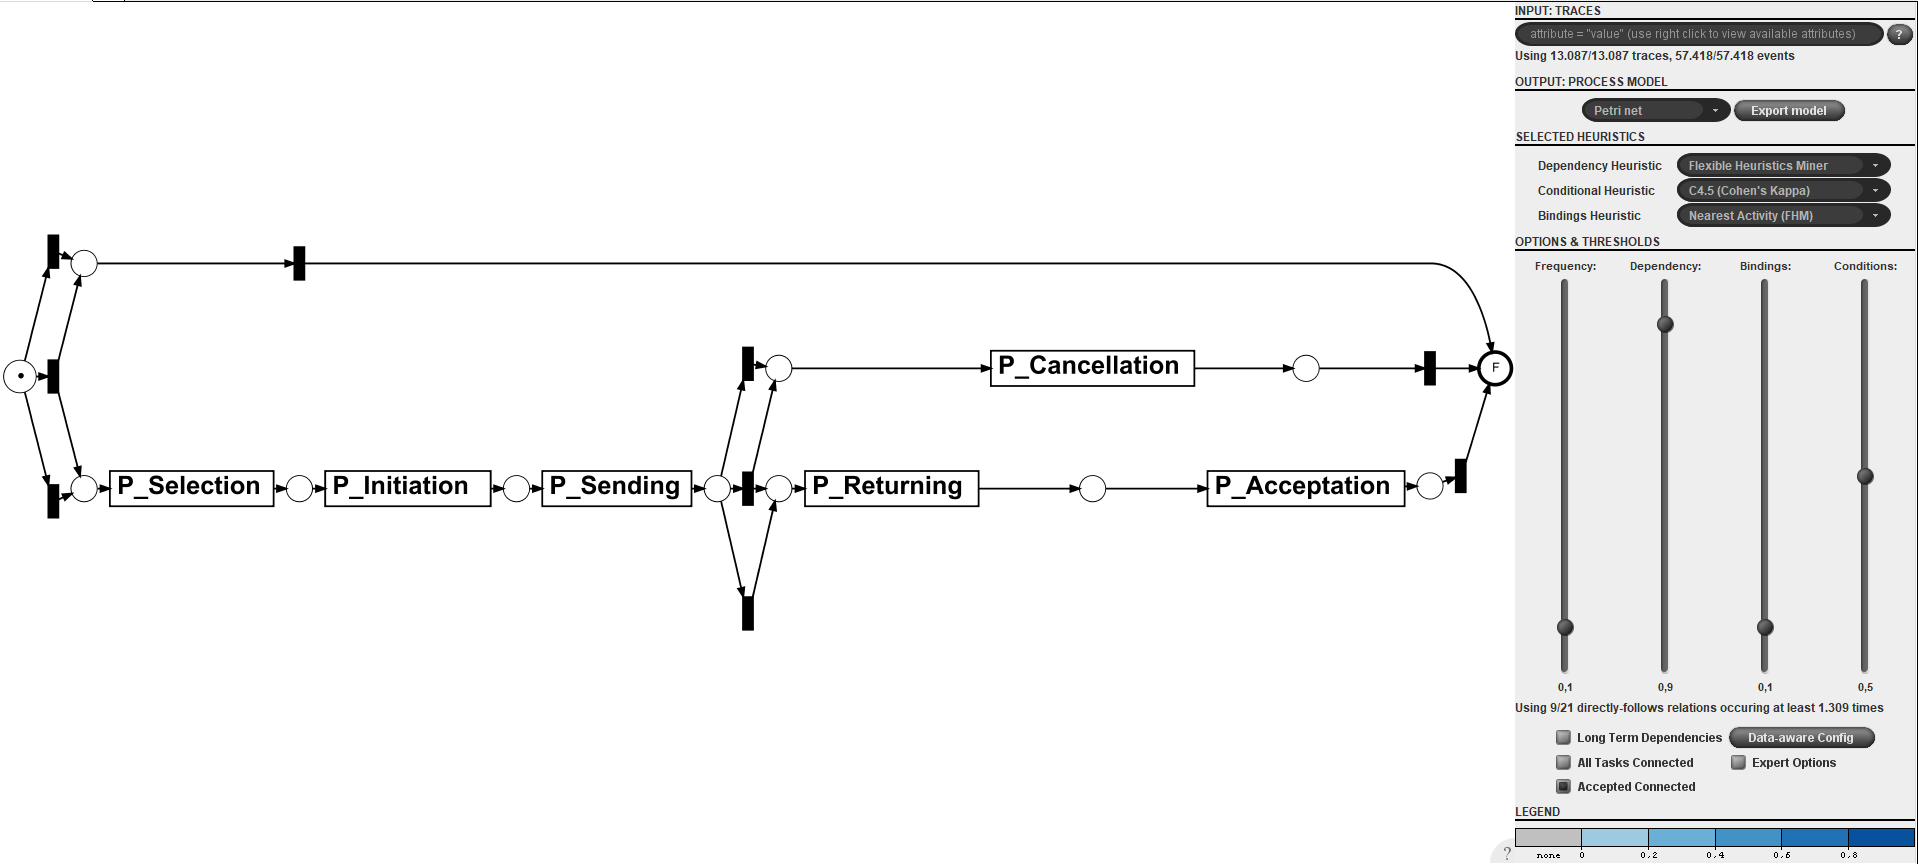
\includegraphics[width=\linewidth]{P_DirectlyFollowedFreq0-1.PNG}
  \caption{Directly followed graph 0.1 frequency}
  \label{fig:P_DFG0-1}
\end{subfigure}
\begin{subfigure}{.4\textwidth}
  \centering
  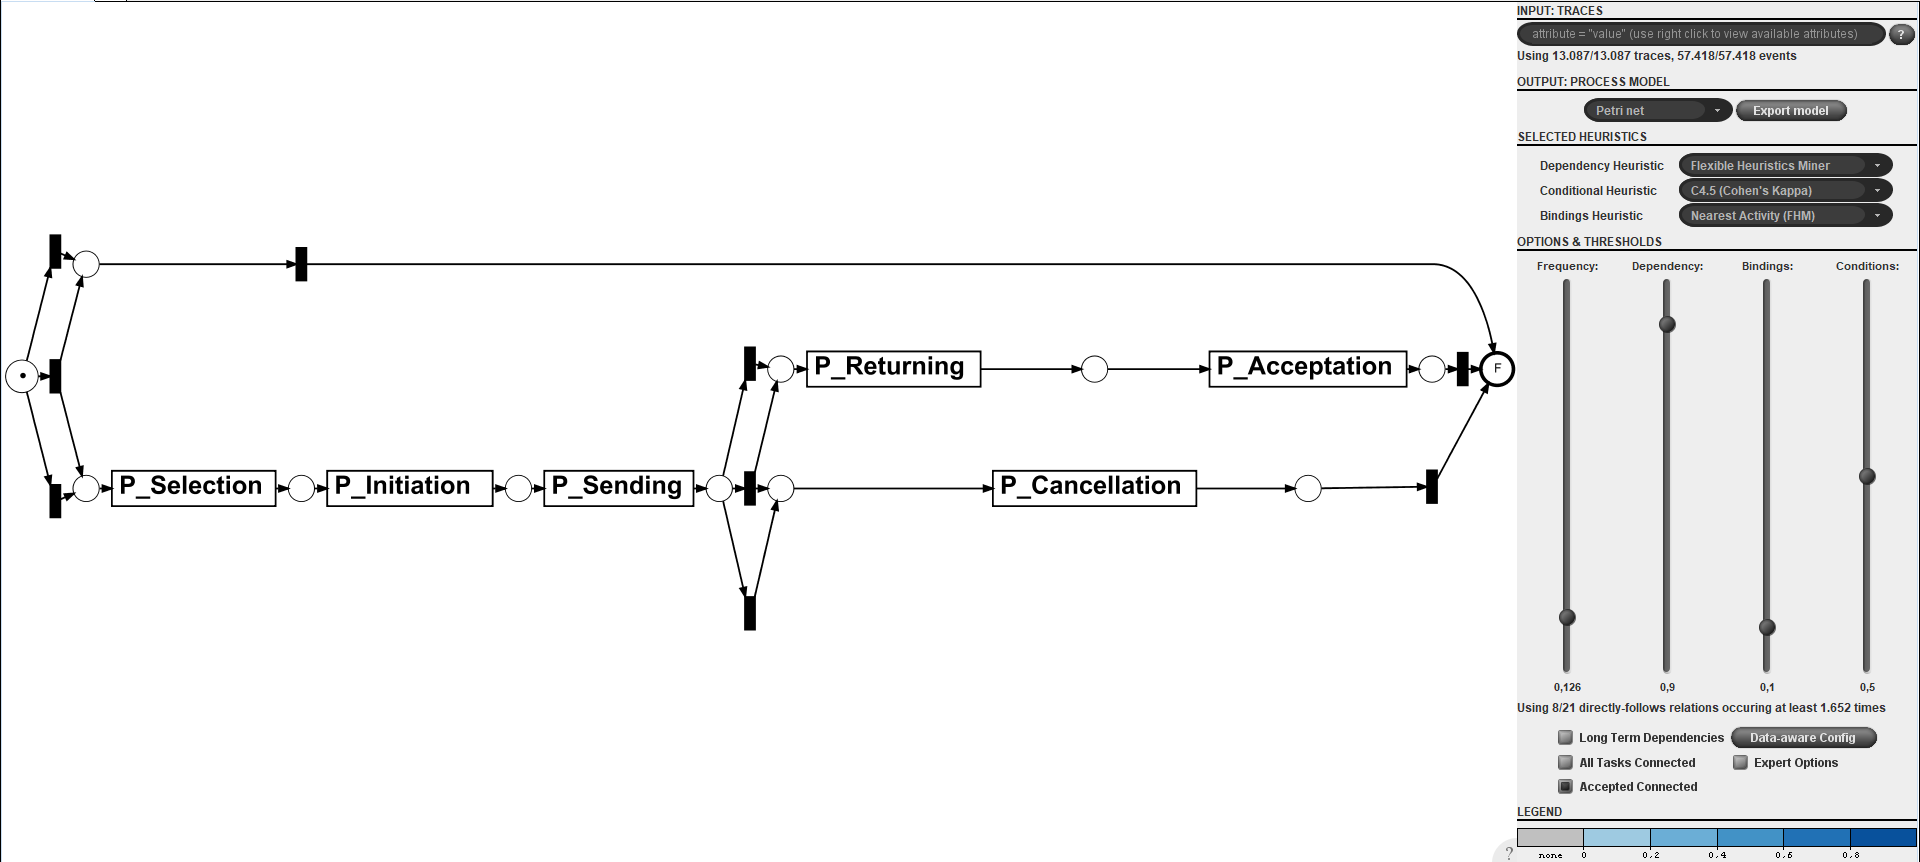
\includegraphics[width=\linewidth]{P_DirectlyFollowedFreq0-126.PNG}
  \caption{Directly followed graph 0.126 frequency}
  \label{fig:P_DFG0-126}
\end{subfigure}
\caption{Considered directly followed graphs}
\label{fig:P_Direct}
\end{figure}

Because of simplicity reasons I piced out of those, figure \ref{fig:P_Direct}, just the 0.051 and 0.1 filtered and checked the conformance and precision for them. 

\begin{figure}[!htbp]
\centering
\begin{subfigure}{.4\textwidth}
  \centering
  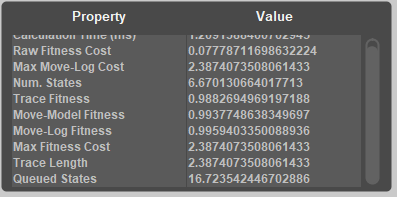
\includegraphics[width=\linewidth]{P_Conformance0-051.PNG}
  \caption{Conformance for 0.051 frequency}
  \label{fig:P_Conf0-051}
\end{subfigure}%
\begin{subfigure}{.4\textwidth}
  \centering
  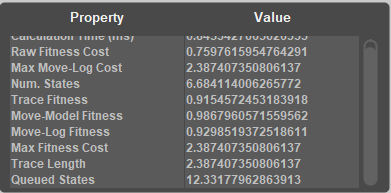
\includegraphics[width=\linewidth]{P_Conformance0-1.PNG}
  \caption{Conformance 0.1}
  \label{fig:P_Conf0-1}
\end{subfigure}
\begin{subfigure}{.4\textwidth}
  \centering
  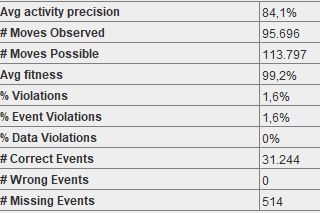
\includegraphics[width=\linewidth]{P_Precision0-051.PNG}
  \caption{Precision for 0.051 as frequency}
  \label{fig:P_Prec0-051}
\end{subfigure}%
\begin{subfigure}{.4\textwidth}
  \centering
  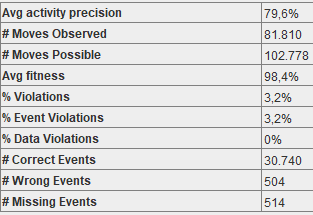
\includegraphics[width=\linewidth]{P_Precision0-1.PNG}
  \caption{Precision for 0.1 as frequency}
  \label{fig:P_Prec0-1}
\end{subfigure}
\caption{Conformance and precision checking}
\label{fig:P_ConfPrec}
\end{figure}


The conformance and precision outcomes, to see in figure \ref{fig:P_ConfPrec}, told me, that the 0.1 frequency model (fitness 91.55\%, precision 80\%) has not a good enough precision. And also the precision of the 0.051 filtering is not really high. So I searched for an other model, which has a similar simplicity as the 0.1 and 0.051 filtered models and has maybe a better performance. The models fullfilling the simplicity criterium had 0.08 or 0.025 frequency filtered.

\begin{figure}[!htbp]
\centering
\begin{subfigure}{0.8\textwidth}
  \centering
  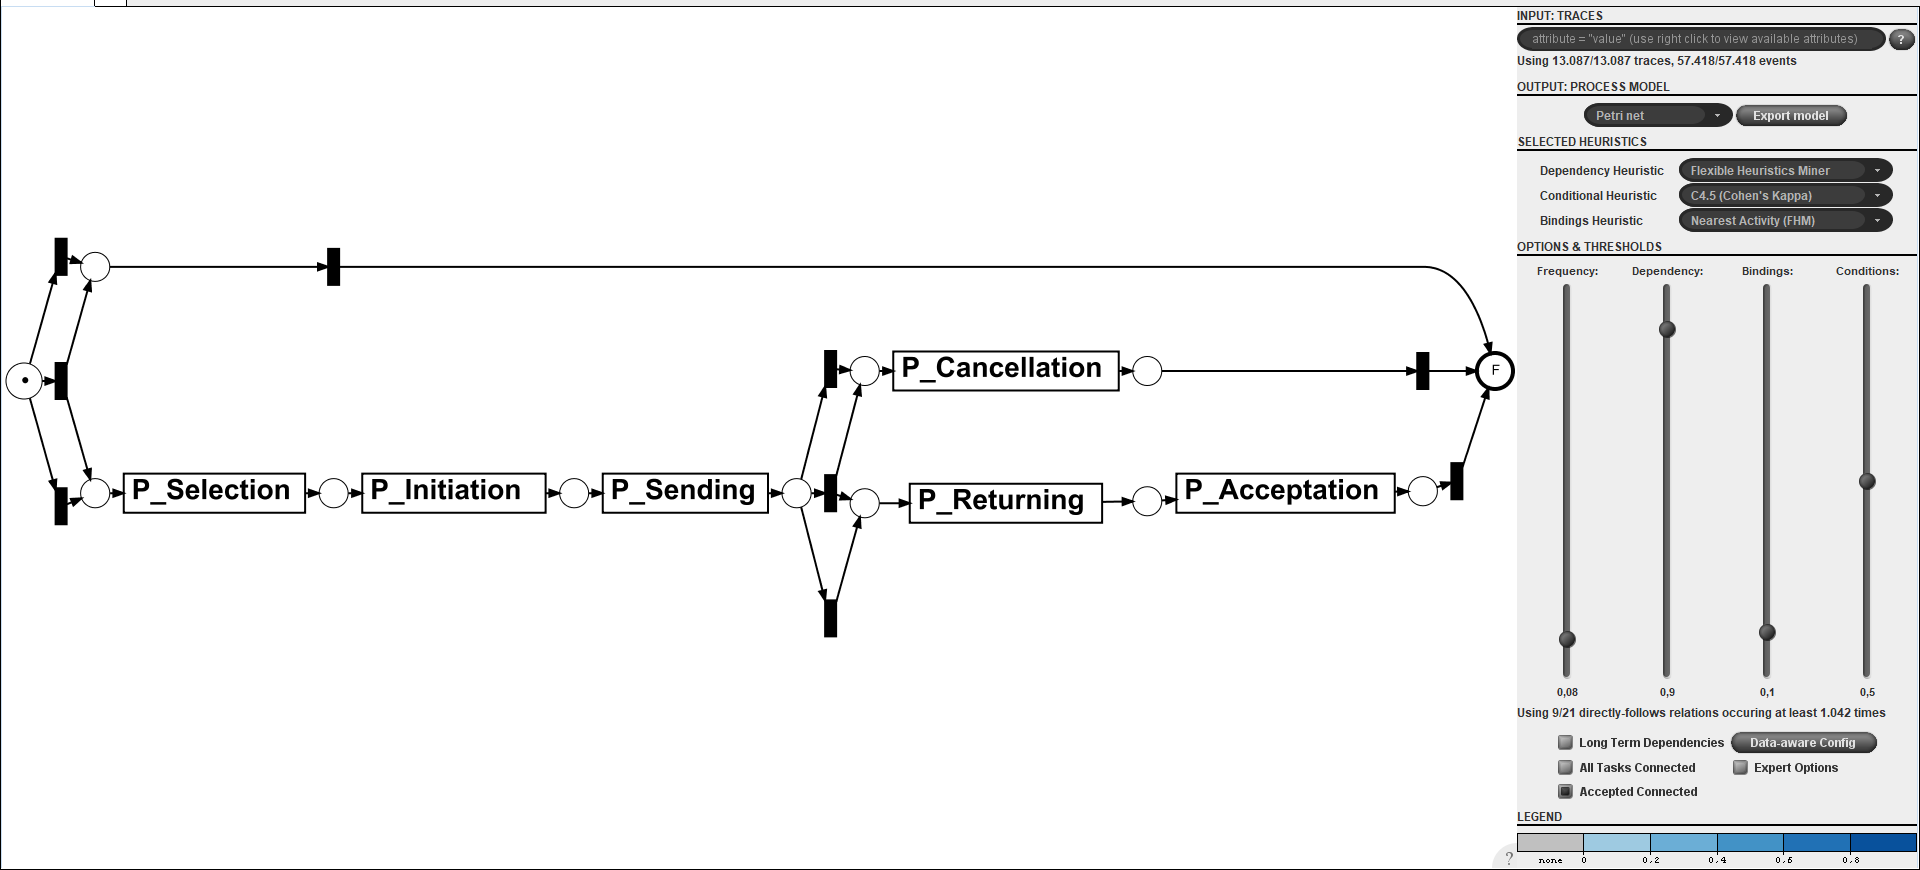
\includegraphics[width=0.3\linewidth]{P_DirectlyFollowedFreq0-08.PNG}
  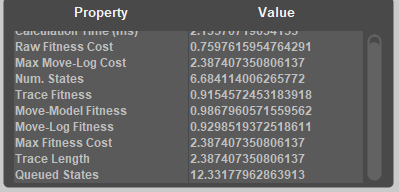
\includegraphics[width=0.3\linewidth]{P_Conformance0-08.PNG}
  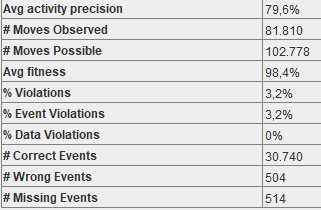
\includegraphics[width=0.3\linewidth]{P_Precision0-08.PNG}
  \caption{0.08 frequency}
  \label{fig:P_0-08}
\end{subfigure}
\begin{subfigure}{0.8\textwidth}
  \centering
  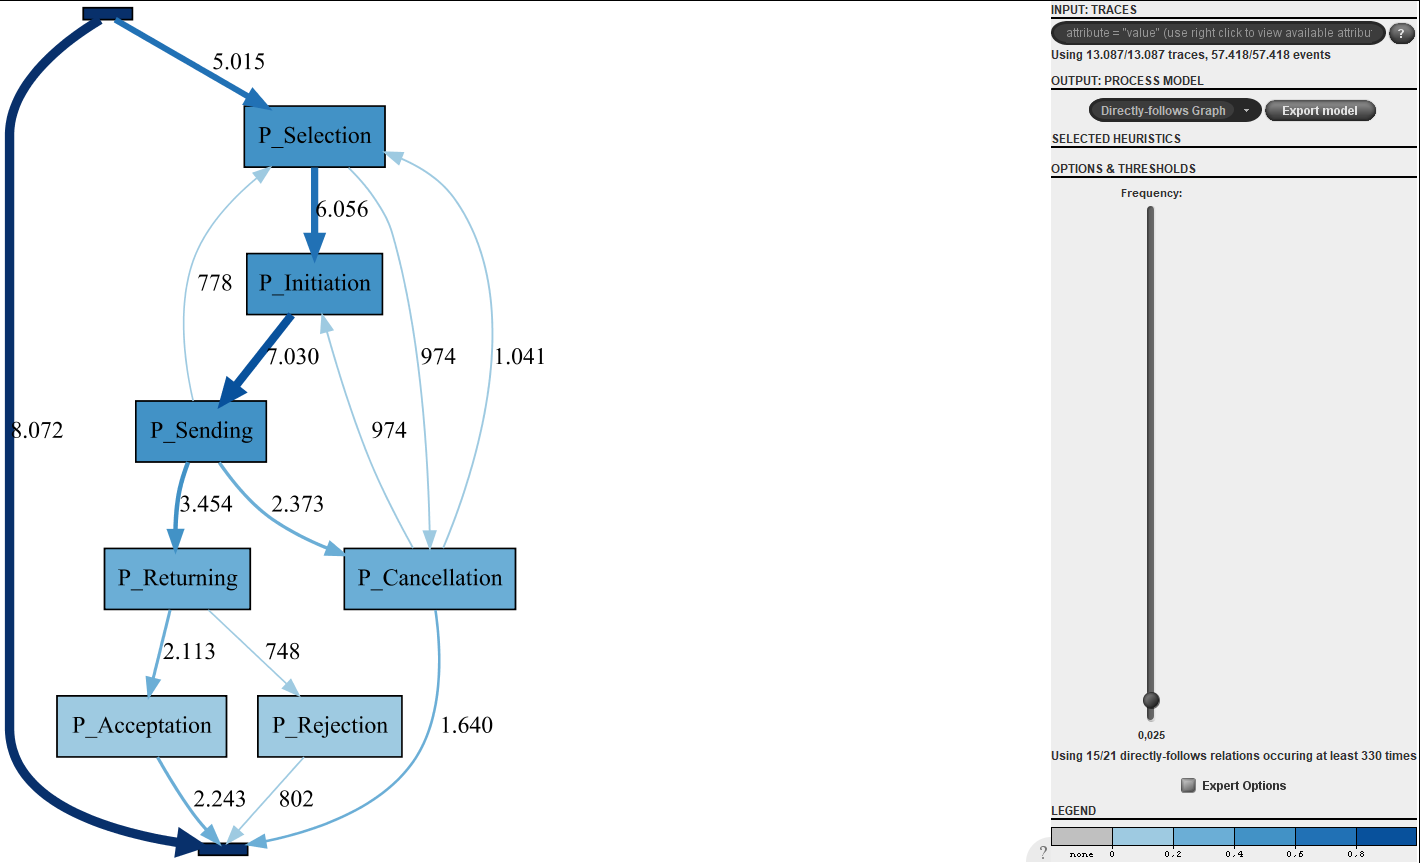
\includegraphics[width=0.3\linewidth]{P_DirectlyFollowedFreq0-025.PNG}
  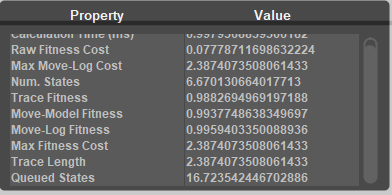
\includegraphics[width=0.3\linewidth]{P_Conformance0-025.PNG}
  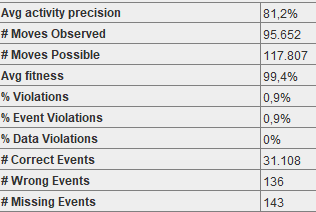
\includegraphics[width=0.3\linewidth]{P_Precision0-025.PNG}
  \caption{0.025 frequency}
  \label{fig:P_0-025}
\end{subfigure}
\caption{Directly followeg graphs, conformance and precision}
\label{fig:P_Direct2}
\end{figure}

After having a look at all results in \ref{fig:P_Direct2} and comparing it with earlier results I chose the model with 0.025. I decided, that the precision is still comparable and better than for 0.051, but it is still a simple enough model to understand the main traces. Choosing a lower frequency threshold made the model to complicated in my opinion.

\subsubsection{Analyzing the explored model}
\begin{wrapfigure}{R}{0.4\textwidth}
  \begin{center}
    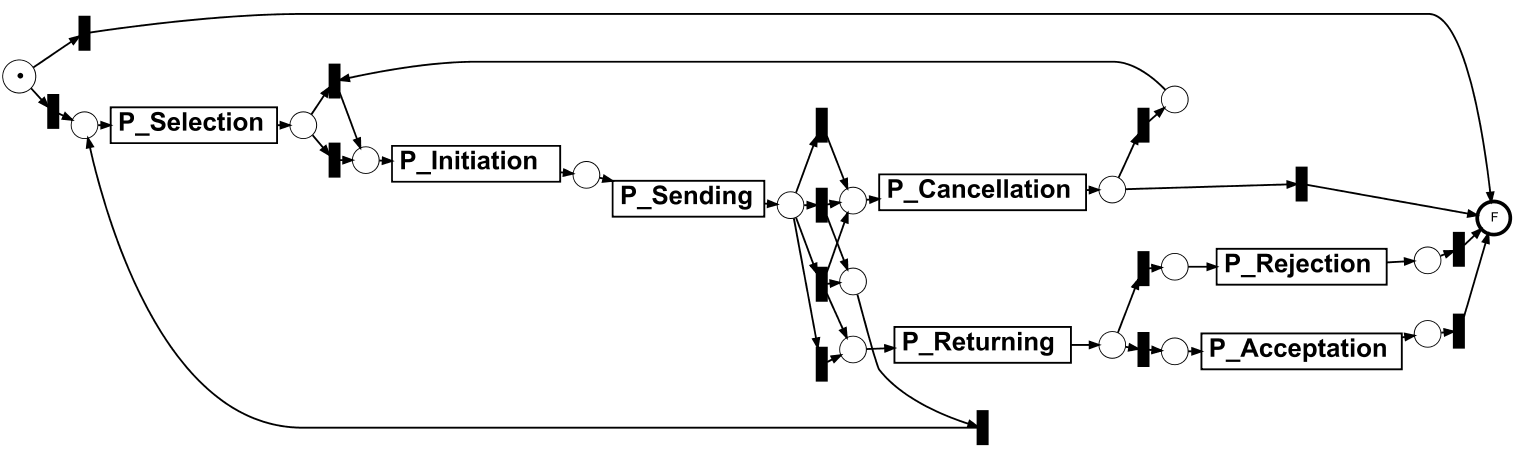
\includegraphics[width = 0.38\textwidth]{P_DirectlyFollowedFreq0-025End.PNG}
  \end{center}
  \caption{0.025 filtered frequency}
\end{wrapfigure}

This model has the conspicuousness, that 8072 cases directly end, but recheck it with the original graph this can be found, too. The other 5015 cases start with "P\_Selection", then the most cases perform the "P\_Initiation" action (6056 cases), while in 974 cases "P\_Selection" is followed by "P\_Cancellation". "P\_Cancellation" builds a loop with "P\_Selection" (10141 cases go to "P\_Selection"). "P\_Initiation" is followed by "P\_Sending" (7030 cases), which has 3 different following actions. In 2373 cases as next action "P\_Cancellation" is performed, so is "P\_Cancellation" in total 3347 times followed like to see in the model. "P\_Cancellation" is in 1640 cases the last action or it leads to "P\_Initiation" (974 times) or "P\_Selection" (1041 times). So it is executed in total 3655 times. "P\_Sending" has also as followed action 778 times "P\_Selection" and in the highest amount of times it is followed by "P\_Returning" (3454 times). "P\_Returning" now lead of to "P\_Acceptation" (2113 cases) or "P\_Rejection" (748 cases). In total "P\_Acceptation" happens in 2243 cases and "P\_Rejection" in 802 cases. Like in the aplication model the differences of cases are a result of the filtering. 

What is special to see is the loop behavior containing "P\_Selection", "P\_Initiation" and "P\_Sending" as loop, or "P\_Selection" and "P\_Cancellation", or "P\_Selection", "P\_Cancellation", "P\_Initiation" and "P\_Sending" in different orders.


\subsection{Combinded Model}
%Models that combine these two models into one showing the lifecycle of the application and the proposal together. Due to the high variability, you should discover one different model for each possible outcome, namely whether the application is finally rejected, cancelled or approved. 

For combinded Models I first filtered the data to have a dataset with all proposal data combined with the application data. This data I filtered with Heuristic filter (all configurations to 100\% and just deciding what the endstate is) with the outcomes/endstates "APP\_rejected" or "APP\_cancelled" or "APP\_approved". I saved them under the names "Filtered P App with approv", "Filtered P App with canc" and "Filtered P App with rej". 

\subsubsection{Endstate APP\_Approved}
Like for approved and proposal I first checked different frequency filter setting to have a first idea, which models fullfill simplicity. Then for every chosen frequency in begin I checked conformance and precision.

\begin{figure}[!htbp]
\centering
\begin{tabular}{c|c|c|c|c|}
\cline{2-5}
& \multicolumn{4}{ c| }{Frequency} \\ \cline{2-5}
& 0 & 0.1 & 0.2 & 0.3 \\ \cline{1-5}
\multicolumn{1}{ |c|  }{Simplicity} 
& - & - & + & ++      \\ \cline{1-5}
\multicolumn{1}{ |c|  }{Fitness}  & 99.84 & 99.47 & 93.93 & 93.93      \\ \cline{1-5}
\multicolumn{1}{ |c| } {Precision} & 93.3 & 94.5 & 91.7 & 94.8  \\ \cline{1-5}
\end{tabular}
\caption{Results for approved as endstate}
\label{tab:ApprovRe}
\end{figure}

Based on the results, \ref{tab:ApprovRe}, I chose the model with 0.3 filtering. This one has a high simplicity, but still has surprisingly good results.
%TODO Maybe all together

\subsubsection{Endstate APP\_Cancelled}

\begin{figure}[!htbp]
\centering
\begin{tabular}{c|c|c|c|}
\cline{2-4}
& \multicolumn{3}{ c| }{Frequency} \\ \cline{2-4}
& 0 & 0.049 & 0.1 \\ \cline{1-4}
\multicolumn{1}{ |c|  }{Simplicity} 
& - & + & ++      \\ \cline{1-4}
\multicolumn{1}{ |c|  }{Fitness}  & 99.96 & 99.39 & 96.84       \\ \cline{1-4}
\multicolumn{1}{ |c| } {Precision} & 92.5 & 91.8 & 94.6   \\ \cline{1-4}
\end{tabular}
\caption{Results for cancelled as endstate}
\label{tab:CancRe}
\end{figure}
Like for APP\_Approved I checked different configurations and based on the results, \ref{tab:CancRe}, I decided to pick 0.1 filtered frequency model. The fitness and precision is still higher than 90\%, but it is also the most simpel model.




\subsubsection{Endstate APP\_Rejected}
The last analysis is of the models ending in APP\_Rejected. In the first step I checked different frequency filters and decided based on simplicity and traceability I had a closer look at 0, 0.025 and 0.1.

\begin{figure}[!htbp]
\centering
\begin{tabular}{c|c|c|c|}
\cline{2-4}
& \multicolumn{3}{ c| }{Frequency} \\ \cline{2-4}
& 0 & 0.025 & 0.1 \\ \cline{1-4}
\multicolumn{1}{ |c|  }{Simplicity} 
& - & + & +++      \\ \cline{1-4}
\multicolumn{1}{ |c|  }{Fitness}  & 1.00 & 99.60 & 96.91       \\ \cline{1-4}
\multicolumn{1}{ |c| } {Precision} & 99.3 & 98.7 & 100   \\ \cline{1-4}
\end{tabular}
\caption{Results for cancelled as endstate}
\label{tab:RejRe}
\end{figure}

Based on \ref{tab:RejRe} I chose 0.1 filtered frequency model as the best. It is really easy to follow and has a good fitness.



\subsubsection{All 3 Models}
\begin{figure}[!htbp]
\centering
\begin{subfigure}{.3\textwidth}
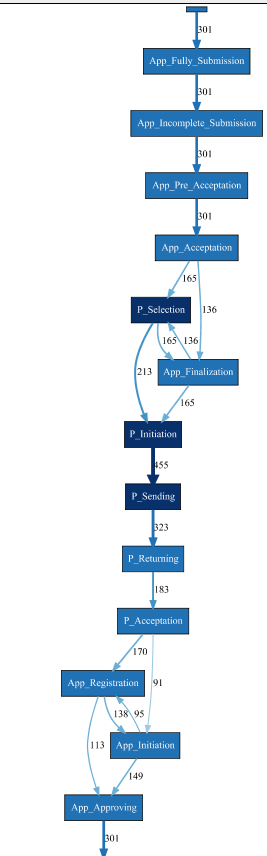
\includegraphics[height=0.3\textheight]{APP_ApprovedDFG0-3.PNG}  
\caption{Endstate APP\_Approved}
\label{fig:ApprovModel}
\end{subfigure}
\begin{subfigure}{.3\textwidth}
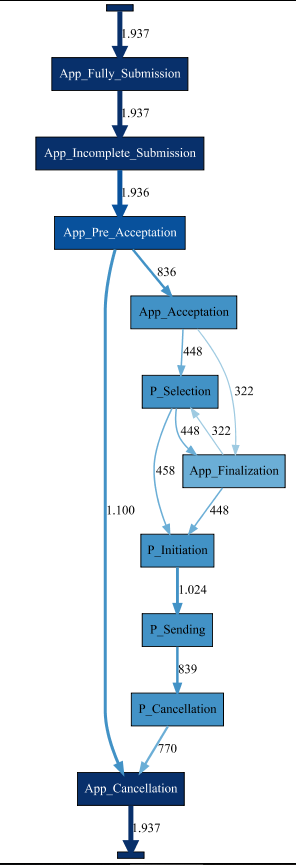
\includegraphics[height=0.3\textheight]{APP_CancDFG0-1.PNG}
\caption{Endstate APP\_Cancelled}
\label{fig:CancModel}
\end{subfigure}
\begin{subfigure}{.3\textwidth}
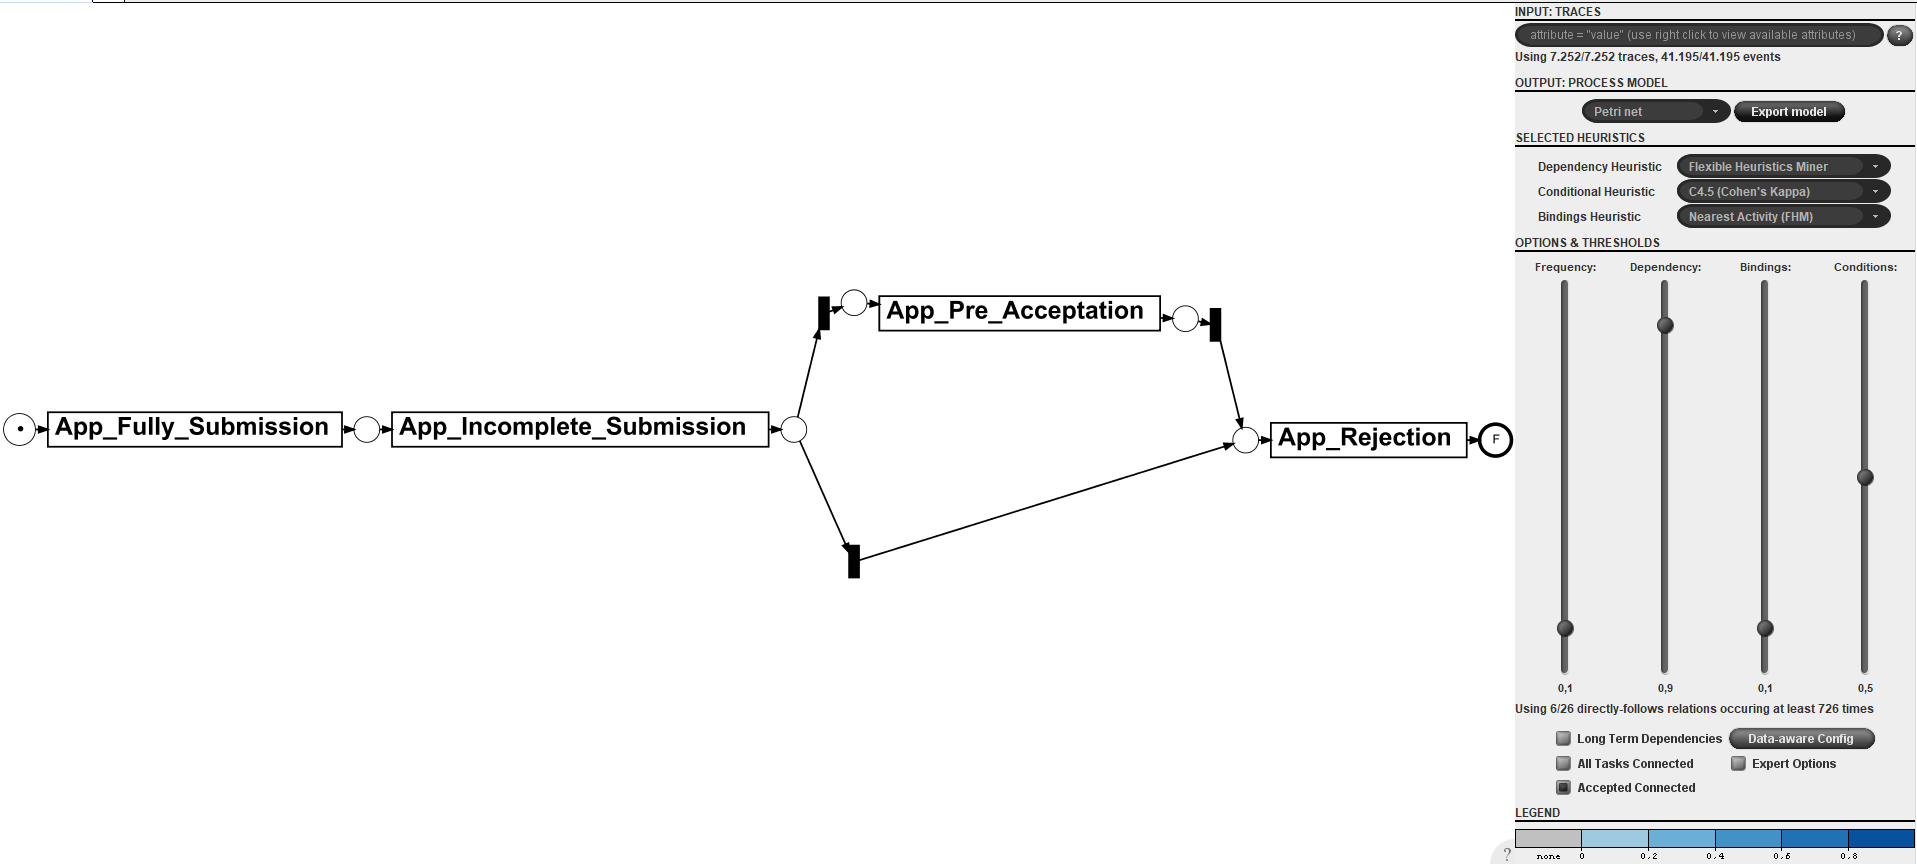
\includegraphics[width=\linewidth]{Rej0-1.PNG}
\caption{Endstate APP\_Rejected}
\label{fig:RejModel}
\end{subfigure}
\caption{Models for the different endstates}
\end{figure}

\subsection{C-net of the proposal process}
%Analyze the C-net of the proposal process and explain it. 

Based on the results of my analysis of the model before I chose the same frequency filtering for the C-net of the proposal process.
\begin{figure}[!htbp]
\centering
\begin{subfigure}{0.8\textwidth}
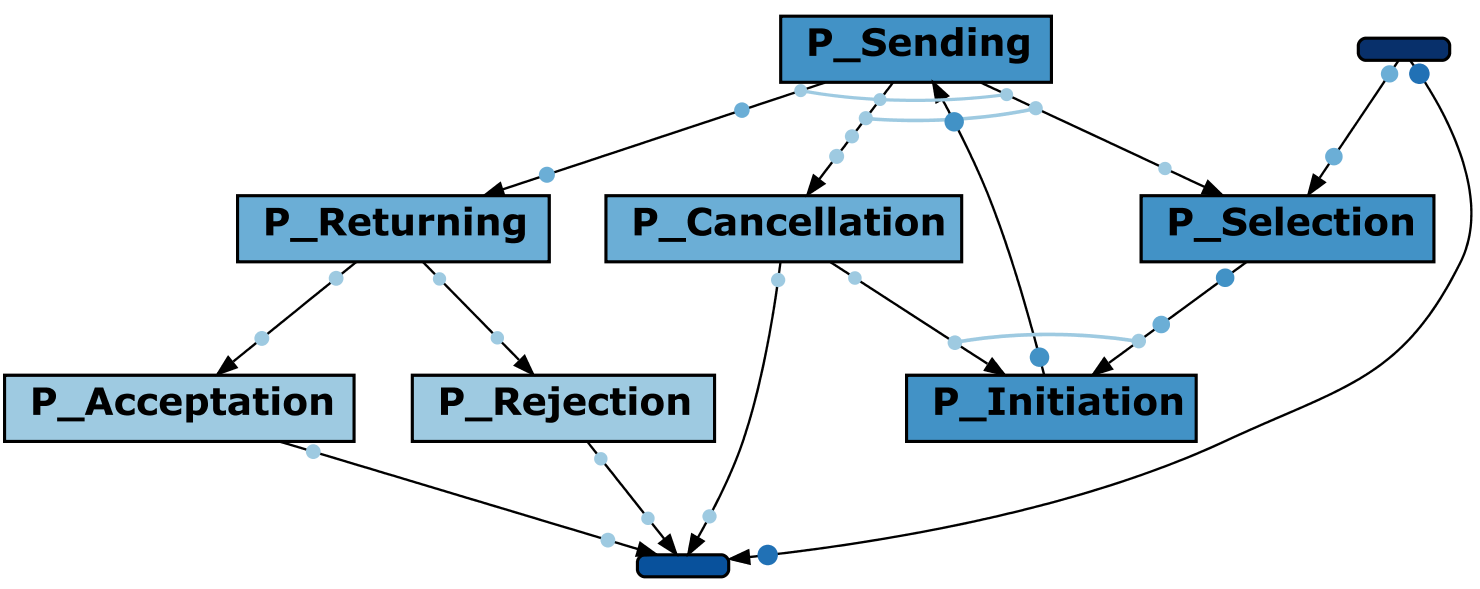
\includegraphics[height = 0.2\textheight]{PropC-Net0-024.PNG}
\caption{C-net with 0.025 filtered frequency}
\label{fig:cnetP0-025}
\end{subfigure}
\begin{subfigure}{0.8\textwidth}
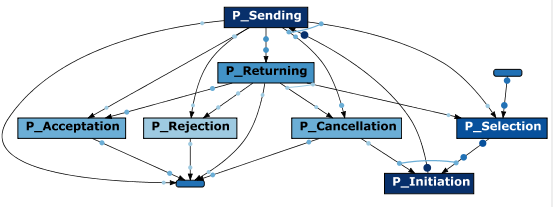
\includegraphics[height = 0.2\textheight]{PropC-Net0.PNG}
\caption{C-net without filtered frequency}
\label{fig:cnetP0}
\end{subfigure}
\caption{C-Nets of the proposal process}
\label{fig:cNetP}
\end{figure}

In \ref{fig:cNetP} I show two C-nets of the proposal process for comparsion. \ref{fig:cnetP0-025} is the one I picked and I will discuss it later in detail. In \ref{fig:cnetP0} the original C-net of the process is to see and obviously it is much more complicated and not so intuitive than the filtered one. 

\subsubsection{Analysis of the C-net}
For simplicity reasons I will not write "P\_" as prefix of every activity.
The first thing I did is having a look at the maximal number of bindings. This is for sending with 6 possible bindings. The input is always from initiation, but there are 4 different outputs possible. Having a look at all possible traces and the corresponding procedures.  Just checking the possible traces shows you, that there are infinite many possible traces, because of a loop between sending and initiation. 
\begin{figure}[!htbp]
\begin{itemize}
	\item Done
	\item Selection \textrightarrow Initiation \textrightarrow Sending \textrightarrow
	\begin{itemize}
	\item  Returning \textrightarrow
	\begin{itemize}
		\item Acceptation \textrightarrow Done
		\item Rejection \textrightarrow Done
	\end{itemize}
	\item ((Cancellation \textrightarrow Selection) or (Selection \textrightarrow Cancellation)) \textrightarrow Initiation \textrightarrow Sending ...
	\item Cancellation \textrightarrow Done
	\end{itemize}
\end{itemize}
\end{figure}

This pathes are also what you would sort of expect. The sending step has the biggest variance in the next step and we have a fixed prefix for the case, that we not directly end.


\subsection{Own Petri net of the proposal process}
%Based on your analysis, create a Petri net of the proposal process by your own. For example, do not consider infrequent paths and also outlier behaviors. 

\subsection{Analysis of the performance of Application and work process}
%Analyze the performance of Application and work process. What are the bottlenecks? What are your recommendations to the company to increase the performance of the process? 